\documentclass{standalone}
\usepackage{tikz}
\usepackage{ctex,siunitx}
\setCJKmainfont{Noto Serif CJK SC}
\usepackage{tkz-euclide}
\usepackage{amsmath}
\usetikzlibrary{patterns, calc,3d}
\usetikzlibrary {decorations.pathmorphing,decorations.pathreplacing,decorations.shapes}
\tikzset{label style/.append style={font=\small}}
\begin{document}
\small
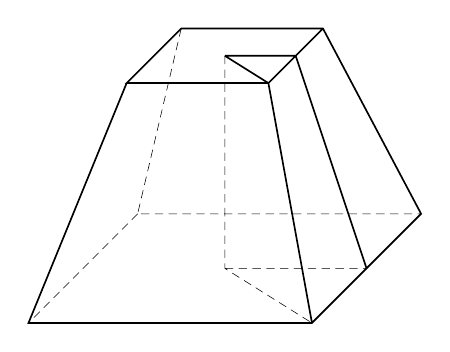
\begin{tikzpicture}[>=latex,scale=0.9,inner sep=1pt]
  \draw[semithick](-1,3,1)--(-2,0,2)--(2,0,2)--(2,0,-2)--(1,3,-1)--(-1,3,-1)--(-1,3,1)--(1,3,1)--(1,3,-1)(2,0,2)--(1,3,1)(1,3,1)--(0,3,0)(0,3,0)--(1,3,0)--(2,0,0);
  \draw[very thin,densely dashed] (-1,3,-1)--(-2,0,-2)--(2,0,-2)(-2,0,-2)--(-2,0,2)(0,3,0)--(0,0,0)--(2,0,2)(0,0,0)--(2,0,0);
\end{tikzpicture}
\end{document}